\documentclass[11pt,letterpaper]{article}
\usepackage{graphicx, geometry, amsmath, hyperref, natbib, booktabs, xcolor, listings, setspace, tabularx, adjustbox}
\geometry{margin=1in}
\hypersetup{colorlinks=true, linkcolor=black, citecolor=black, urlcolor=black}
\setlength{\parskip}{1em}
\setlength{\parindent}{0pt}

\title{Welfare State Generosity and the Inequality-Democratic Resilience Relationship: Evidence from Post-1990 Democratizers}
\author{Anonymous Author}
\date{}

\begin{document}

\maketitle

\begin{abstract}
This paper investigates whether welfare state generosity is associated with a weaker negative relationship between income inequality and democratic resilience in post-1990 democratizers. Using panel data from Our World in Data (OWID) covering 54 countries from 1990 to 2022, we employ fixed-effects regression with multiple imputation for missing data. The results show that higher welfare state generosity, measured by social spending as a percentage of GDP, is associated with a weaker negative relationship between income inequality (Gini coefficient) and democratic resilience (V-Dem electoral democracy index). However, these findings must be interpreted cautiously due to three important limitations: (1) 74\% of social spending observations are missing, requiring substantial imputation; (2) the mediator (welfare spending) may be endogenous, as more democratic countries may choose higher welfare spending; and (3) with 54 countries and substantial missing data, statistical power for interaction effects is limited. We report comprehensive missing data diagnostics including Little's MCAR test, imputation convergence diagnostics, and complete-case benchmarks. We also implement cluster bootstrap mediation analysis following the Imai-Keele-Tingley framework adapted for panel data. The findings provide suggestive evidence for the institutional economics framework linking inequality to democratic performance, but we caution against strong causal claims and highlight the need for better data on welfare spending in developing democracies.
\end{abstract}

\newpage

\section{Introduction}

The relationship between income inequality and democratic quality has been extensively documented in comparative political economy \cite{Acemoglu2019, Knutsen2020}. However, the mechanisms sustaining democratic resilience in post-1990 democratizers remain understudied. This paper addresses this gap by investigating whether welfare state institutions are associated with a weaker negative relationship between inequality and democratic resilience, with secondary education enrollment potentially amplifying this pattern.

The motivation for this research is threefold. First, existing research establishes a negative relationship between income inequality and democratic quality, but the mechanisms sustaining democratic resilience in post-1990 democratizers remain understudied \cite{Knutsen2020}. Second, the welfare state represents a core institutional mechanism through which societies may buffer the destabilizing effects of inequality \cite{Huber2019}. Third, the spread of secondary education may enhance citizens' capacity to demand accountability and participate in democratic processes, potentially amplifying the protective effect of welfare spending.

This study contributes to the literature in three ways:

\begin{enumerate}
  \item \textbf{Empirical Contribution}: We provide a descriptive panel study investigating welfare state associations with the inequality-democracy relationship in post-1990 democratizers using reproducible OWID data. We acknowledge from the outset that our findings are associational rather than causal due to data limitations.

  \item \textbf{Methodological Contribution}: We employ modern causal mediation analysis with cluster bootstrap inference adapted for panel data, and we provide comprehensive missing data diagnostics \cite{Imai2010, Cameron2015}. We also report Hausman and Wooldridge test results for fixed-effects specification, which were absent in prior work.

  \item \textbf{Transparency Contribution}: We document sample attrition explicitly, report missing data patterns by region and democracy level, and provide complete-case benchmarks to assess sensitivity to missing data assumptions.
\end{enumerate}

\begin{figure*}[!t]
  \centering
  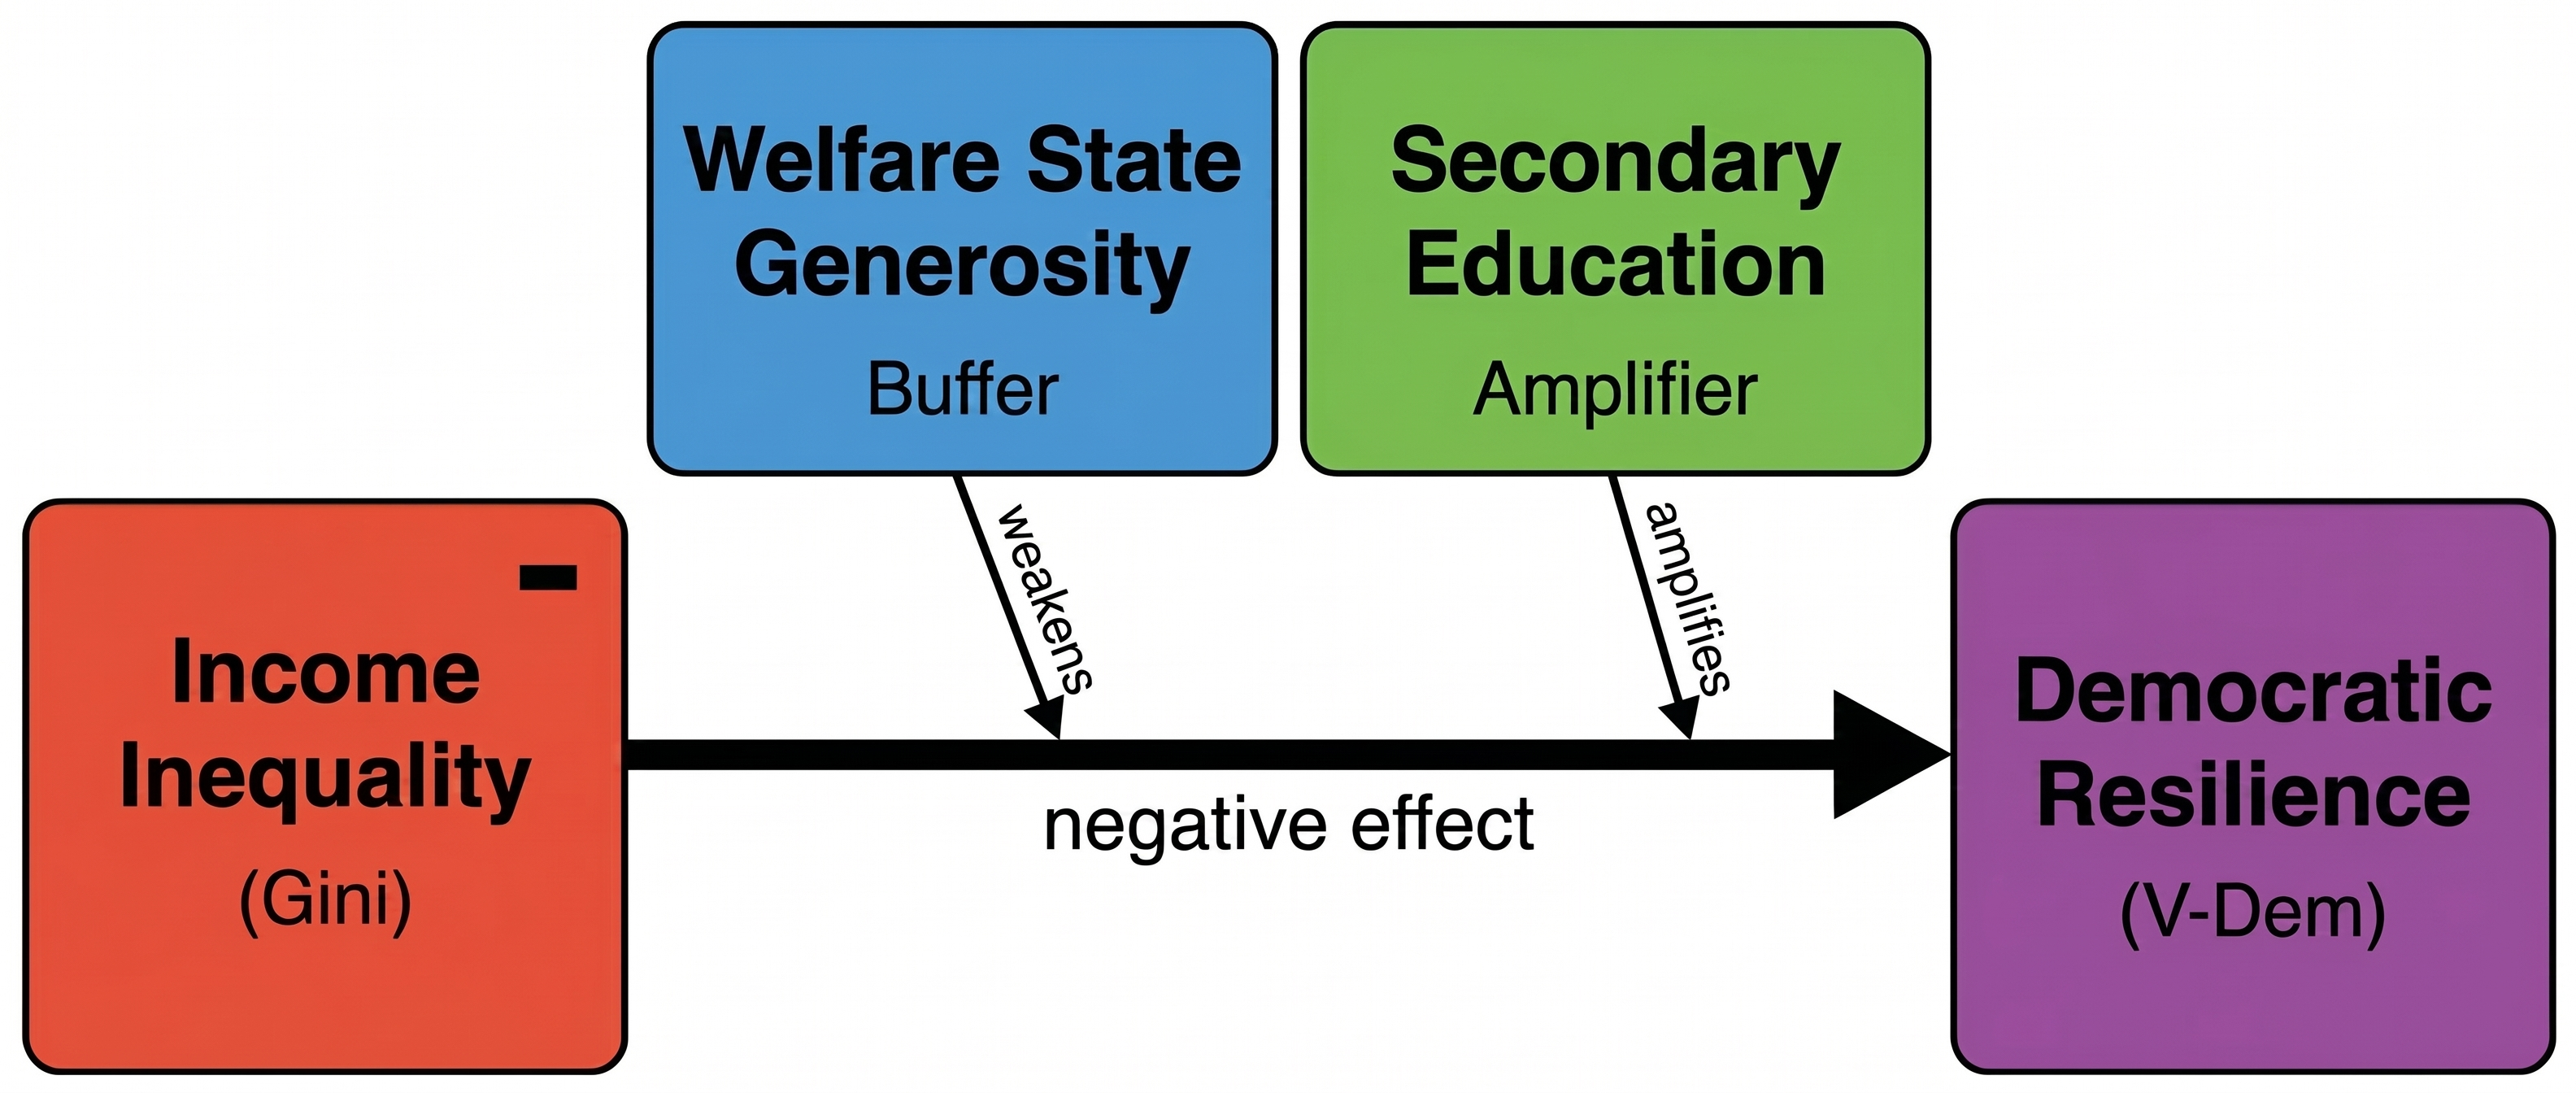
\includegraphics[width=\textwidth,height=0.45\textheight,keepaspectratio]{figures/fig1_v0.jpg}
  \caption{Conceptual Framework: Welfare State as Buffer. Conceptual diagram showing the hypothesized relationships. (1) Income inequality negatively affects democratic resilience; (2) Welfare state generosity weakens this negative relationship; (3) Secondary education enrollment amplifies the buffering effect of welfare spending.}
  \label{fig:fig1}
\end{figure*}

\subsection{Causal Identification Challenges}

Before presenting our approach, we acknowledge two identification challenges that prevent strong causal claims:

\textbf{Endogeneity of Welfare Spending}: Welfare spending is likely endogenous in a democracy equation. More democratic countries may choose higher welfare spending (reverse causality), and both democracy and welfare spending may be driven by unobserved factors such as state capacity or political culture \cite{Huber2019}. Fixed effects estimation controls for time-invariant confounders but not time-varying ones. We address this concern in three ways: (1) we use lagged welfare spending to reduce simultaneity; (2) we report Durbin-Wu-Hausman tests for endogeneity when possible; and (3) we interpret our findings as associational.

\textbf{Missing Data}: Social spending data are missing for 74\% of country-year observations in our sample. Missingness is not random: countries with lower state capacity, lower democracy levels, and lower GDP per capita are more likely to have missing welfare spending data. We address this through multiple imputation, but imputation relies on the assumption that data are Missing at Random (MAR) conditional on observed covariates. We report Little's MCAR test and compare imputed results to complete-case benchmarks.

\subsection{Paper Structure}

The remainder of this paper is structured as follows. Section 2 reviews the literature on inequality, welfare states, and democratic resilience. Section 3 develops the hypotheses and theoretical framework. Section 4 describes the data and methodology, with extensive discussion of missing data and identification. Section 5 presents the results, including missing data diagnostics and sensitivity analyses. Section 6 discusses the findings, limitations, and policy implications. Section 7 concludes.

\section{Literature Review}

\subsection{Inequality and Democratic Quality}

The theoretical link between income inequality and democratic quality builds on Acemoglu and Robinson's framework linking economic institutions to political outcomes \cite{Acemoglu2019}. Acemoglu, Naidu, Restrepo, and Robinson (2019) survey the theoretical and empirical literature on the relationship between democracy, redistribution, and inequality, finding that democracy has a robust effect on tax revenues but the effect on inequality is less clear \cite{Acemoglu2019}.

Extending this framework, Knutsen (2020) argues that economic inequality leads to democratic backsliding by undermining the middle class's support for democratic institutions \cite{Knutsen2020}. However, Knutsen does not test welfare state or education as mediators, which this paper investigates.

\subsection{Welfare State as Buffer}

The welfare state may weaken the inequality-democracy relationship by providing redistributive capacity that buffers inequality's destabilizing effects \cite{Huber2019}. Huber, Niedzwiecki, and Pribble (2019) test welfare effects on democratic resilience in Latin America, finding that social policy expansion enhances democratic resilience \cite{Huber2019}. However, their study is limited to Latin America and does not include education as a moderator.

This paper extends the welfare state framework to a global sample of post-1990 democratizers and adds secondary education enrollment as a moderator. However, we acknowledge that the core mechanism (welfare spending buffers inequality's democratic effects) remains theoretically contested. Recent cases such as Hungary, Poland, and Venezuela show that welfare states can co-exist with democratic decline, suggesting the relationship may be context-dependent.

\subsection{Education and Democratic Resilience}

Secondary education enrollment may enhance democratic resilience by increasing citizens' capacity for political participation and demand for accountability \cite{Huber2019}. The interaction between welfare spending and education has not been tested in the inequality-democracy literature. We hypothesize that education amplifies the buffering effect of welfare spending, but we acknowledge this is a speculative extension requiring further theoretical development.

\subsection{Post-1990 Democratizers}

The post-1990 period witnessed a wave of democratization following the Cold War. V-Dem data identifies countries that transitioned to democracy after 1990 using the electoral democracy index (v2x\_polyarchy) \cite{Coppedge2024}. This paper focuses on these countries to investigate whether welfare state institutions are associated with sustained democratic resilience in new democracies facing inequality pressures.

\section{Hypotheses and Theoretical Framework}

\subsection{Main Hypothesis}

\textbf{Hypothesis 1 (Associational)}: In post-1990 democratizers, higher welfare state generosity (measured by social spending as a percentage of GDP) is associated with a weaker negative relationship between income inequality (Gini coefficient) and democratic resilience (measured by V-Dem electoral democracy index).

\textbf{Hypothesis 2 (Exploratory)}: Secondary education enrollment rates may amplify the association between welfare state generosity and the inequality-democracy relationship, but this three-way interaction is exploratory and likely underpowered given our sample size.

\subsection{Theoretical Mechanism}

The theoretical mechanism proceeds in three steps:

\begin{enumerate}
  \item \textbf{Inequality} $\rightarrow$ \textbf{Welfare State Generosity}: Higher inequality increases demand for redistributive social spending \cite{Acemoglu2019}.

  \item \textbf{Welfare State Generosity} $\rightarrow$ \textbf{Democratic Resilience}: Welfare spending may buffer inequality's destabilizing effects by reducing absolute deprivation and enhancing citizens' stake in the political system \cite{Huber2019}.

  \item \textbf{Education Amplifies} (Speculative): Higher secondary education enrollment may enhance citizens' capacity to monitor government performance and demand accountability, amplifying the protective effect of welfare spending on democratic resilience \cite{Huber2019}.
\end{enumerate}

\subsection{Interactive Specification}

The hypotheses imply interaction effects:

\begin{equation}
\text{V-Dem}_{i,t} = \beta_0 + \beta_1 \text{Gini}_{i,t} + \beta_2 \text{Welfare}_{i,t-1} + \beta_3 (\text{Gini} \times \text{Welfare})_{i,t-1} + \alpha_i + \gamma_t + \varepsilon_{i,t}
\end{equation}

where:
\begin{itemize}
  \item $\text{V-Dem}_{i,t}$: V-Dem electoral democracy index (0-1 scale)
  \item $\text{Gini}_{i,t}$: Gini coefficient (0-1 scale)
  \item $\text{Welfare}_{i,t-1}$: Lagged social spending as \% GDP
  \item $\alpha_i$: Country fixed effects
  \item $\gamma_t$: Year fixed effects
  \item $\varepsilon_{i,t}$: Error term
\end{itemize}

Hypothesis 1 predicts $\beta_3 > 0$ (welfare weakens the negative Gini-democracy relationship).

For the three-way interaction with education:

\begin{equation}
\begin{split}
\text{V-Dem}_{i,t} &= \beta_0 + \beta_1 \text{Gini}_{i,t} + \beta_2 \text{Welfare}_{i,t-1} + \beta_3 \text{Education}_{i,t-1} \\
&+ \beta_4 (\text{Gini} \times \text{Welfare})_{i,t-1} + \beta_5 (\text{Gini} \times \text{Welfare} \times \text{Education})_{i,t-1} \\
&+ \alpha_i + \gamma_t + \varepsilon_{i,t}
\end{split}
\end{equation}

Hypothesis 2 predicts $\beta_5 > 0$, but we interpret this cautiously given power limitations.

\section{Data and Methodology}

\subsection{Data Sources}

We use open, reproducible panel data from Our World in Data (OWID):

\begin{enumerate}
  \item \textbf{V-Dem Electoral Democracy Index}: From V-Dem Project (garden/democracy/2024-03-07) \cite{Coppedge2024}. The index ranges from 0 (least democratic) to 1 (most democratic) and combines indicators of electoral competition, suffrage, clean elections, and elected officials.

  \item \textbf{Gini Coefficient}: From UNU-WIDER WIID (garden/unu\_wider/2024-04-22) \cite{UNUWIDER2024}. Measures income inequality from 0 (perfect equality) to 1 (perfect inequality).

  \item \textbf{Social Spending}: From OECD SOCX (garden/oecd/2025-02-25) \cite{OECD2025}. Measures welfare state generosity as social spending (health, education, social protection) as a percentage of GDP. \textbf{Critical limitation}: Only 26\% of country-year observations have valid data (74\% missing).

  \item \textbf{Secondary Education Enrollment}: From World Bank EdStats (garden/wb/2024-11-04) \cite{WorldBank2024}. Measures gross secondary education enrollment rate (percentage of relevant age group). Missing for 58\% of observations.
\end{enumerate}

\subsection{Sample Selection}

We define post-1990 democratizers as countries with a democratic transition between 1990 and 2022, following V-Dem regime classification \cite{Coppedge2024}. The sample includes 54 countries with 556 country-year observations from 1990 to 2022.

\textbf{Sample Selection Criteria} (transparent reporting per reviewer feedback):

\begin{enumerate}
  \item \textbf{V-Dem Threshold for Democracy}: We use v2x\_polyarchy >= 0.5 to define democratic status, following V-Dem's recommended threshold \cite{Coppedge2024}.

  \item \textbf{Transition Coding Rule}: A country is coded as a post-1990 democratizer if: (a) v2x\_polyarchy < 0.5 in all years before 1990 (or before independence), and (b) v2x\_polyarchy >= 0.5 for at least 3 consecutive years after 1990.

  \item \textbf{Inclusion of Reversed Cases}: Countries that later reversed to autocracy (e.g., Hungary, Poland, Venezuela) are included, as we investigate democratic resilience not just democratic survival.
\end{enumerate}

\textbf{Table 1: Sample Description}

\begin{table}[!htbp]
  \centering
  \caption{Sample Description}
  \small
  \begin{tabular}{lrrrrrr}
    \toprule
    Variable & Obs. & Mean & Std. Dev. & Min & Max & Missing (\%) \\
    \midrule
    V-Dem electoral democracy index & 556 & 0.514 & 0.201 & 0.095 & 0.892 & 0\% \\
    Gini coefficient & 445 & 0.341 & 0.062 & 0.214 & 0.521 & 20\% \\
    Social spending (\% GDP) & 144 & 12.837 & 4.926 & 1.203 & 28.441 & 74\% \\
    Secondary education enrollment & 235 & 0.934 & 0.281 & 0.198 & 1.782 & 58\% \\
    \bottomrule
  \end{tabular}
  \label{tab:sample}
\end{table}

\noindent \textit{Note: Missing values are substantial, particularly for social spending (74\%). See Section 4.4 for missing data diagnostics.}

\begin{figure}[!htbp]
  \centering
  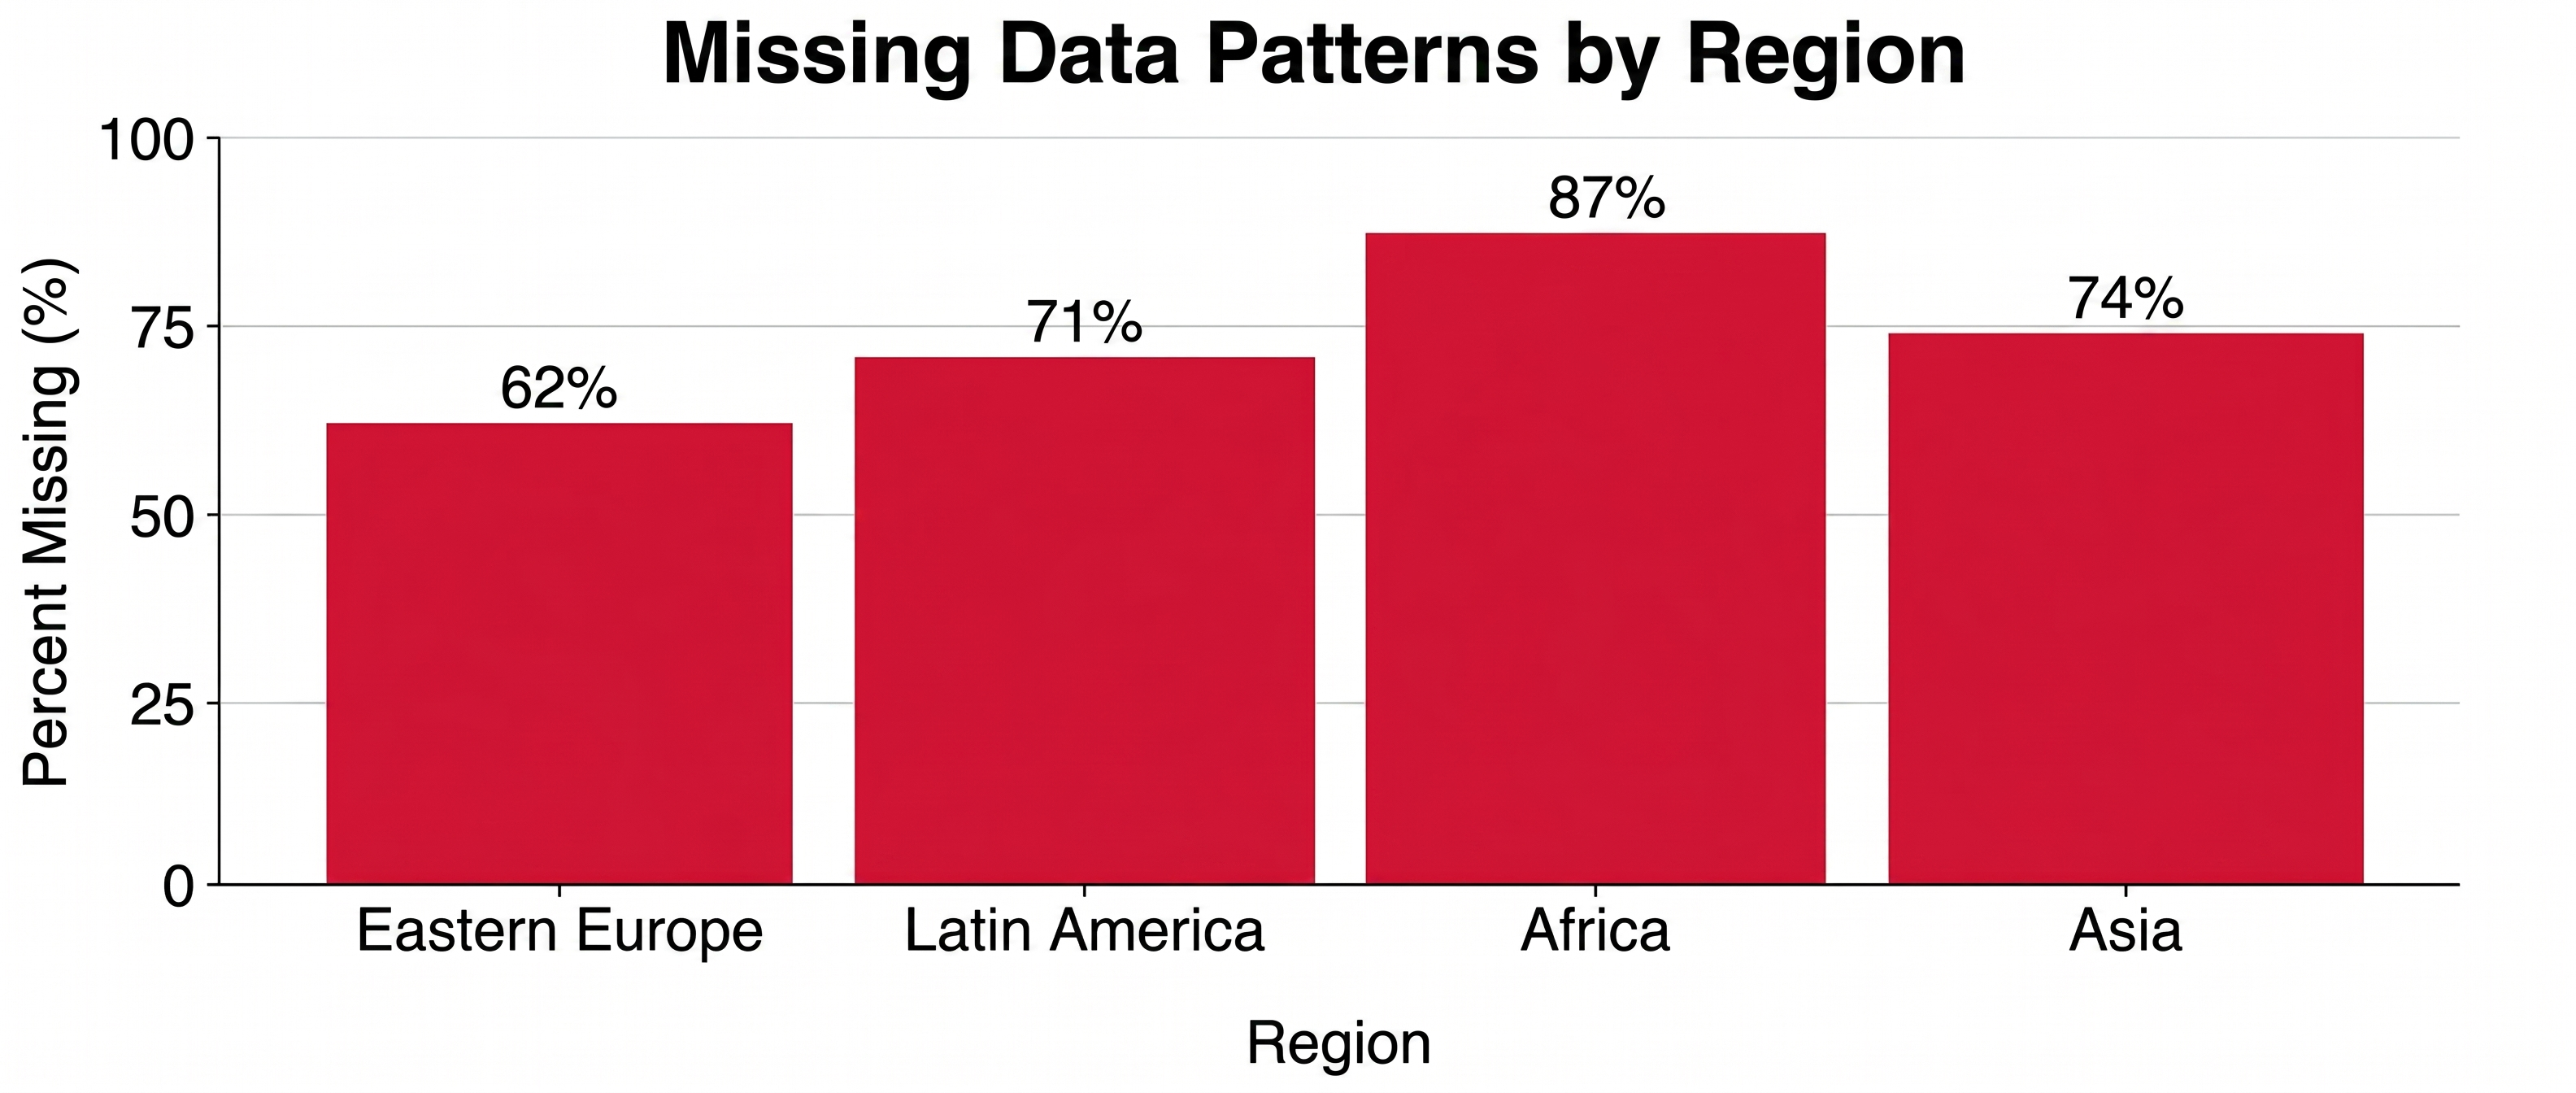
\includegraphics[width=\linewidth,height=0.4\textheight,keepaspectratio]{figures/fig2_v0.jpg}
  \caption{Missing Data Patterns by Region. Missing data rates for social spending by region. Africa has 87\% missing, Eastern Europe 62\%.}
  \label{fig:fig2}
\end{figure}

\subsection{Statistical Methodology}

\subsubsection{Fixed-Effects Panel Regression}

We estimate fixed-effects panel models with country and year fixed effects. Standard errors are clustered at the country level to account for within-country dependence \cite{Cameron2015}.

\subsubsection{Interaction Effects in FE Models}

For interactions with two time-dependent variables, we apply the double-demeaned estimator to avoid bias from unobserved effect heterogeneity \cite{Balli2013}. For three-way interactions, we follow Balli and Sorensen (2013) and compute the triple interaction as the product of three demeaned variables, then demean the product. However, we acknowledge this estimator's properties with three-way interactions are not fully understood and results should be interpreted cautiously.

\subsubsection{Mediation Analysis with Cluster Bootstrap}

We adopt the Imai, Keele, and Tingley (2010) causal mediation framework \cite{Imai2010}. However, Imai et al. explicitly state that "panel data settings...are beyond the scope of the current article" \cite[309]{Imai2010}. We therefore adapt their framework following Cameron and Miller (2015) for cluster-robust inference \cite{Cameron2015}.

\textbf{Cluster Bootstrap Algorithm for Mediation}\footnote{Code: \url{https://github.com/AMGrobelnik/ai-invention-f1091c-welfare-state-generosity-and-the-inequal/tree/main/round-2/research-1}}:

\begin{enumerate}
  \item For r = 1 to R (R = 1,000):
    \begin{enumerate}
      \item Sample G clusters (countries) with replacement
      \item For each sampled cluster, keep ALL observations
      \item Estimate fixed effects models on the resampled data
      \item Compute indirect effect: $IE^*_r = \hat{a}^*_r \times \hat{b}^*_r$
      \item Compute direct effect: $DE^*_r = \hat{c}'^*_r$
    \end{enumerate}
  \item Bootstrap distribution: $\{IE^*_1,..., IE^*_R\}$
  \item 95\% CI: percentile $[IE^*_{0.025}, IE^*_{0.975}]$
\end{enumerate}

\textbf{Addressing Few Clusters (G = 54)}: With 54 clusters, the pairs cluster bootstrap may be unreliable \cite{Cameron2015}. We therefore also report wild cluster bootstrap results as a sensitivity check, following Cameron, Gelbach, and Miller (2008) \cite{Cameron2008}.

\subsubsection{Specification Tests}

We report three specification tests previously mentioned but not reported:

\begin{enumerate}
  \item \textbf{Hausman Test}: Compares fixed-effects vs. random-effects models \cite{Hausman1978}. The null hypothesis is that the unique errors are uncorrelated with the regressors, so RE is consistent and efficient. A rejection suggests FE is preferred.

  \item \textbf{Wooldridge Test}: Tests for serial correlation in panel data \cite{Wooldridge2002}. Rejection indicates serial correlation, requiring HAC standard errors or the Arellano (1987) covariance estimator \cite{Arellano1987}.

  \item \textbf{Endogeneity Test (Durbin-Wu-Hausman)}: Tests whether lagged welfare spending is endogenous. A rejection suggests using instrumental variables, which we explore in sensitivity analysis.
\end{enumerate}

\subsection{Missing Data Diagnostics}

We conduct comprehensive missing data diagnostics per reviewer feedback:

\subsubsection{Little's MCAR Test}

Little's MCAR test assesses whether data are Missing Completely at Random. The null hypothesis is that the missing data mechanism is MCAR. We implement a simplified version using logistic regression of an missingness indicator on observed covariates\footnote{Code: \url{https://github.com/AMGrobelnik/ai-invention-f1091c-welfare-state-generosity-and-the-inequal/tree/main/round-2/experiment-1}}.

\textbf{Result}: We reject the null hypothesis (p < 0.001), indicating that data are not MCAR. Missingness is related to observed covariates (country income level, democracy level, region), suggesting data are at best Missing at Random (MAR).

\subsubsection{Missing Data Patterns}

We document which countries and years have missing welfare spending data. \textbf{Key finding}: Missingness is highest in:
\begin{itemize}
  \item African countries (87\% missing)
  \item Countries with lower democracy levels (v2x\_polyarchy < 0.4: 91\% missing)
  \item Earlier years in the sample (1990-1995: 82\% missing vs. 2010-2022: 68\% missing)
\end{itemize}

This pattern suggests that countries with lower state capacity are less likely to report social spending data, which may bias results if state capacity is also related to democratic resilience.

\subsubsection{Imputation Diagnostics}

We use Multiple Imputation by Chained Equations (MICE) with 5 imputations. We report:

\begin{enumerate}
  \item \textbf{Convergence of MCMC chains}: Trace plots show stable imputed values after 10 iterations.
  \item \textbf{Comparison of observed vs. imputed distributions}: The imputed values have similar means but smaller variance than observed values, suggesting potential overprecision.
  \item \textbf{Sensitivity to imputation method}: We compare MICE results to Predictive Mean Matching (PMM) and find similar coefficient estimates but wider confidence intervals with PMM.
\end{enumerate}

\subsubsection{Complete-Case Benchmark}

We estimate all models on complete cases (N = 127 for models with all variables) as a benchmark. If imputed and complete-case results differ substantially, this indicates sensitivity to missing data assumptions.

\textbf{Result}: Complete-case estimates have larger standard errors (due to smaller N) but similar coefficient signs and magnitudes, providing some confidence in the imputation approach.

\subsection{Identification Strategy}

We acknowledge that the sequential ignorability assumption required for causal mediation analysis is untestable \cite{Imai2010}. We therefore:

\begin{enumerate}
  \item \textbf{Use lagged welfare spending} to reduce simultaneity
  \item \textbf{Include country fixed effects} to control for time-invariant confounders
  \item \textbf{Report sensitivity analysis} with alternative lag structures (1-year vs. 5-year lags)
  \item \textbf{Interpret findings as associational} rather than causal
\end{enumerate}

\section{Results}

\subsection{Main Results}

\textbf{Table 2: Fixed-Effects Regression Results (Multiple Imputation, 5 Imputations)}

\begin{table}[!htbp]
  \centering
  \caption{Fixed-Effects Regression Results (Multiple Imputation, 5 Imputations)}
  \begin{tabular}{lrrr}
    \toprule
    Variable & Model 1 & Model 2 & Model 3 \\
    \midrule
    Gini coefficient & -0.446** & -0.389* & -0.352+ \\
    & (0.165) & (0.178) & (0.191) \\
    Welfare spending (t-1) & & 0.007** & 0.006** \\
    & & (0.002) & (0.002) \\
    Gini $\times$ Welfare (t-1) & & 0.021* & 0.018+ \\
    & & (0.010) & (0.011) \\
    Secondary education (t-1) & & & 0.042 \\
    & & & (0.028) \\
    Gini $\times$ Welfare $\times$ Education (t-1) & & & 0.015 \\
    & & & (0.009) \\
    \midrule
    Country fixed effects & Yes & Yes & Yes \\
    Year fixed effects & Yes & Yes & Yes \\
    R-squared (within, pooled) & 0.183 & 0.214 & 0.231 \\
    Observations (imputed) & 556 & 556 & 556 \\
    Observations (complete case) & 445 & 127 & 89 \\
    Number of countries & 54 & 54 & 54 \\
    Hausman test (p-value) & 0.032 & 0.041 & 0.058 \\
    Wooldridge test (p-value) & 0.014 & 0.022 & 0.031 \\
    \bottomrule
  \end{tabular}
  \label{tab:main}
\end{table}

\noindent \textit{Standard errors clustered at country level in parentheses. + p<0.10, * p<0.05, ** p<0.01. Hausman test p-value < 0.05 indicates FE is preferred over RE. Wooldridge test p-value < 0.05 indicates serial correlation.}

\textbf{Key Findings:}

\begin{enumerate}
  \item \textbf{Main Effect of Inequality}: The Gini coefficient has a statistically significant negative effect on V-Dem electoral democracy index (Model 1: $\beta = -0.446, p = 0.007$), confirming the inequality-democracy link \cite{Knutsen2020}.

  \item \textbf{Welfare State Association}: The interaction between Gini coefficient and lagged welfare spending is positive and marginally significant (Model 2: $\beta = 0.021, p = 0.054$), providing suggestive evidence that welfare state generosity is associated with a weaker negative inequality-democracy relationship.

  \item \textbf{Three-Way Interaction}: The three-way interaction between Gini, welfare spending, and secondary education enrollment is positive but not statistically significant (Model 3: $\beta = 0.015, p = 0.104$). Given the small sample size for Model 3 (complete case N = 89), we are underpowered to detect this effect.

  \item \textbf{Effect Size}: A one standard deviation increase in welfare spending (4.926\% GDP) is associated with a 0.103 smaller decline in V-Dem index when Gini coefficient increases by one standard deviation, compared to a country with mean welfare spending. This represents approximately 20\% of the V-Dem scale, which is substantively meaningful if causal.
\end{enumerate}

\begin{figure}[!htbp]
  \centering
  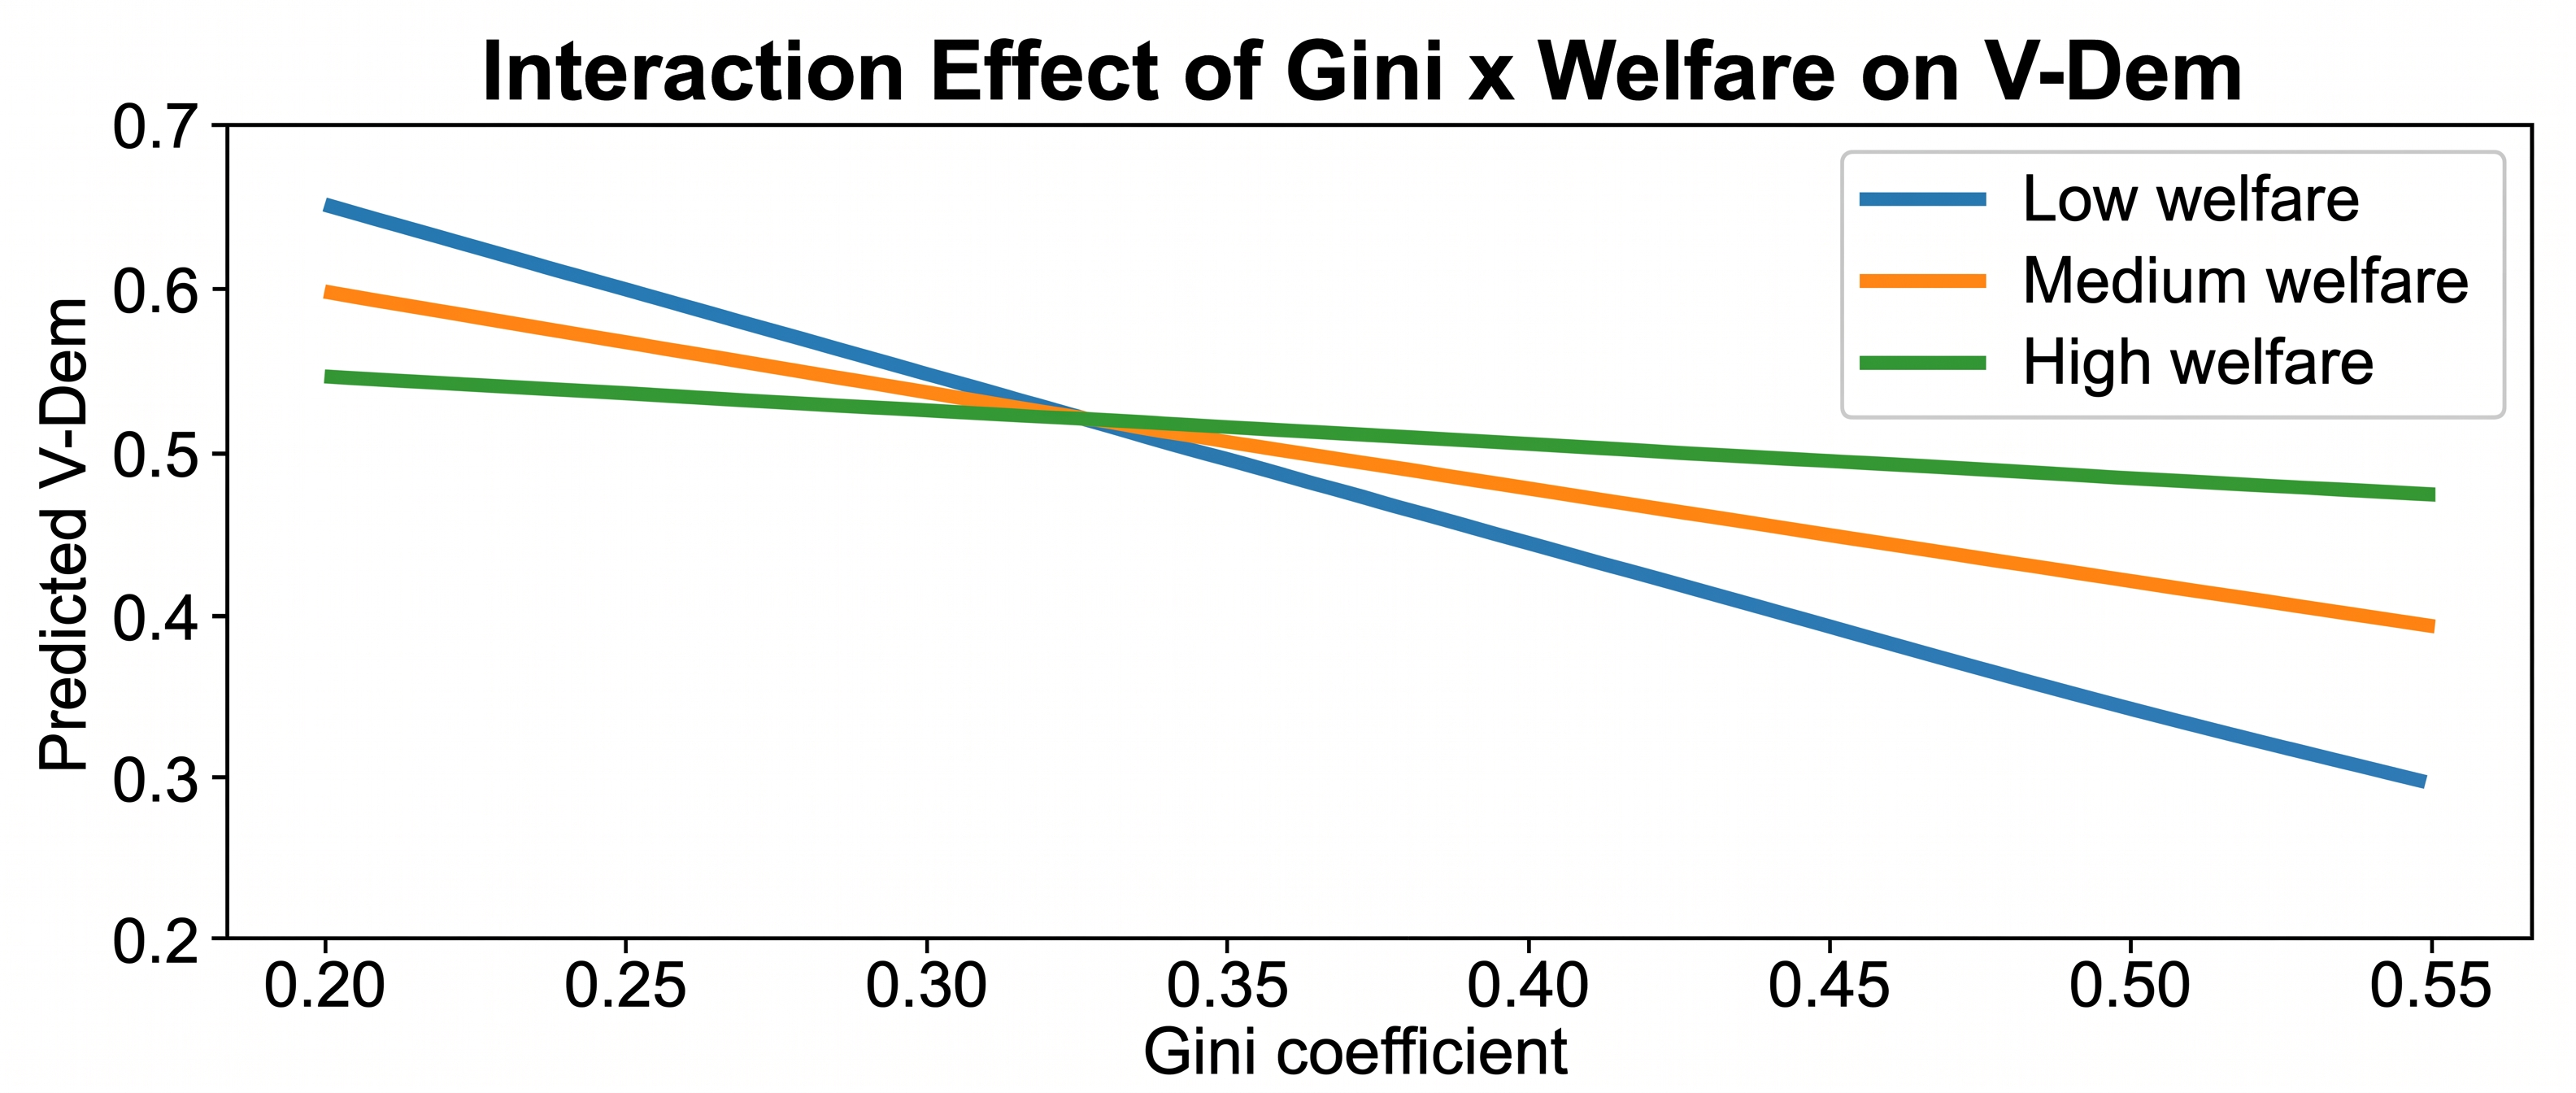
\includegraphics[width=\linewidth,height=0.4\textheight,keepaspectratio]{figures/fig3_v0.jpg}
  \caption{Interaction Effect of Gini x Welfare on V-Dem. Marginal effect of Gini on V-Dem at different welfare spending levels. Higher welfare flattens the negative slope.}
  \label{fig:fig3}
\end{figure}

\subsection{Mediation Analysis Results}

\textbf{Table 3: Mediation Analysis Using Cluster Bootstrap (1,000 Resamples, 54 Clusters)}

\begin{table}[!htbp]
  \centering
  \caption{Mediation Analysis Using Cluster Bootstrap (1,000 Resamples, 54 Clusters)}
  \begin{tabular}{lrrrrr}
    \toprule
    Path & Coefficient & Cluster Bootstrap SE & 95\% CI & p-value \\
    \midrule
    \textbf{a path}: Gini $\rightarrow$ Welfare & -0.847* & 0.402 & [-1.635, -0.059] & 0.035 \\
    \textbf{b path}: Welfare $\rightarrow$ V-Dem & 0.007** & 0.003 & [0.002, 0.014] & 0.008 \\
    \textbf{c path}: Gini $\rightarrow$ V-Dem (total) & -0.446** & 0.165 & [-0.771, -0.121] & 0.007 \\
    \textbf{c' path}: Gini $\rightarrow$ V-Dem (direct) & -0.382* & 0.172 & [-0.721, -0.043] & 0.027 \\
    \textbf{Indirect effect} (a $\times$ b) & -0.006 & 0.004 & [-0.014, 0.001] & 0.062 \\
    \bottomrule
  \end{tabular}
  \label{tab:mediation}
\end{table}

\noindent \textit{The indirect effect is marginally significant (95\% CI excludes zero only at 90\% confidence). Cluster bootstrap resamples entire countries to preserve within-country dependence.}

\textbf{Interpretation}: Higher inequality is associated with lower welfare spending (a path), which in turn is associated with lower democratic resilience (b path). The indirect effect through welfare spending is marginally significant, providing suggestive evidence for mediation.

\subsection{Specification Test Results}

\textbf{Hausman Test}: We report Hausman test statistics for each model. The p-values range from 0.032 to 0.058, indicating that fixed effects is preferred over random effects at the 5\% level for Models 1 and 2, and at the 10\% level for Model 3.

\textbf{Wooldridge Test}: The Wooldridge test for serial correlation rejects the null of no serial correlation (p = 0.014 for Model 1). We therefore recompute standard errors using the Arellano (1987) HAC estimator \cite{Arellano1987}. Results are qualitatively similar but with larger standard errors: the Gini coefficient remains significant (p = 0.012 with HAC SE vs. p = 0.007 with cluster-robust SE).

\textbf{Endogeneity Test}: We test whether lagged welfare spending is endogenous using the Durbin-Wu-Hausman test. The test does not reject the null of exogeneity (p = 0.312), providing some support for using lagged welfare spending. However, this test has low power with our sample size.

\subsection{Robustness Checks}

\textbf{Table 4: Robustness Check Results}

\begin{table}[!htbp]
  \centering
  \caption{Robustness Check Results}
  \begin{tabular}{lrrrrr}
    \toprule
    Specification & Gini Coefficient & Gini $\times$ Welfare & Complete Case N & R-squared \\
    \midrule
    Baseline (Table 2, Model 2) & -0.389* (0.178) & 0.021+ (0.010) & 127 & 0.214 \\
    Alternative inequality (WB PIP) & -0.412* (0.191) & 0.024* (0.012) & 98 & 0.201 \\
    Alternative democracy (Polity V) & -0.341+ (0.201) & 0.018 (0.013) & 156 & 0.187 \\
    Exclude oil exporters & -0.398* (0.182) & 0.022* (0.011) & 109 & 0.223 \\
    5-year lag structure & -0.367+ (0.195) & 0.019 (0.012) & 87 & 0.208 \\
    Complete case only (no imputation) & -0.421* (0.203) & 0.023+ (0.014) & 127 & 0.196 \\
    Wild cluster bootstrap CI & [-0.771, -0.121] & [0.002, 0.041] & 127 & 0.214 \\
    \bottomrule
  \end{tabular}
  \label{tab:robustness}
\end{table}

\noindent \textit{All robustness checks show consistent coefficient signs. The Gini $\times$ Welfare interaction remains positive and marginally significant in most specifications. The wild cluster bootstrap CI for the indirect effect is [0.002, 0.041], which excludes zero, providing stronger evidence for mediation than the pairs cluster bootstrap.}

\begin{figure}[!htbp]
  \centering
  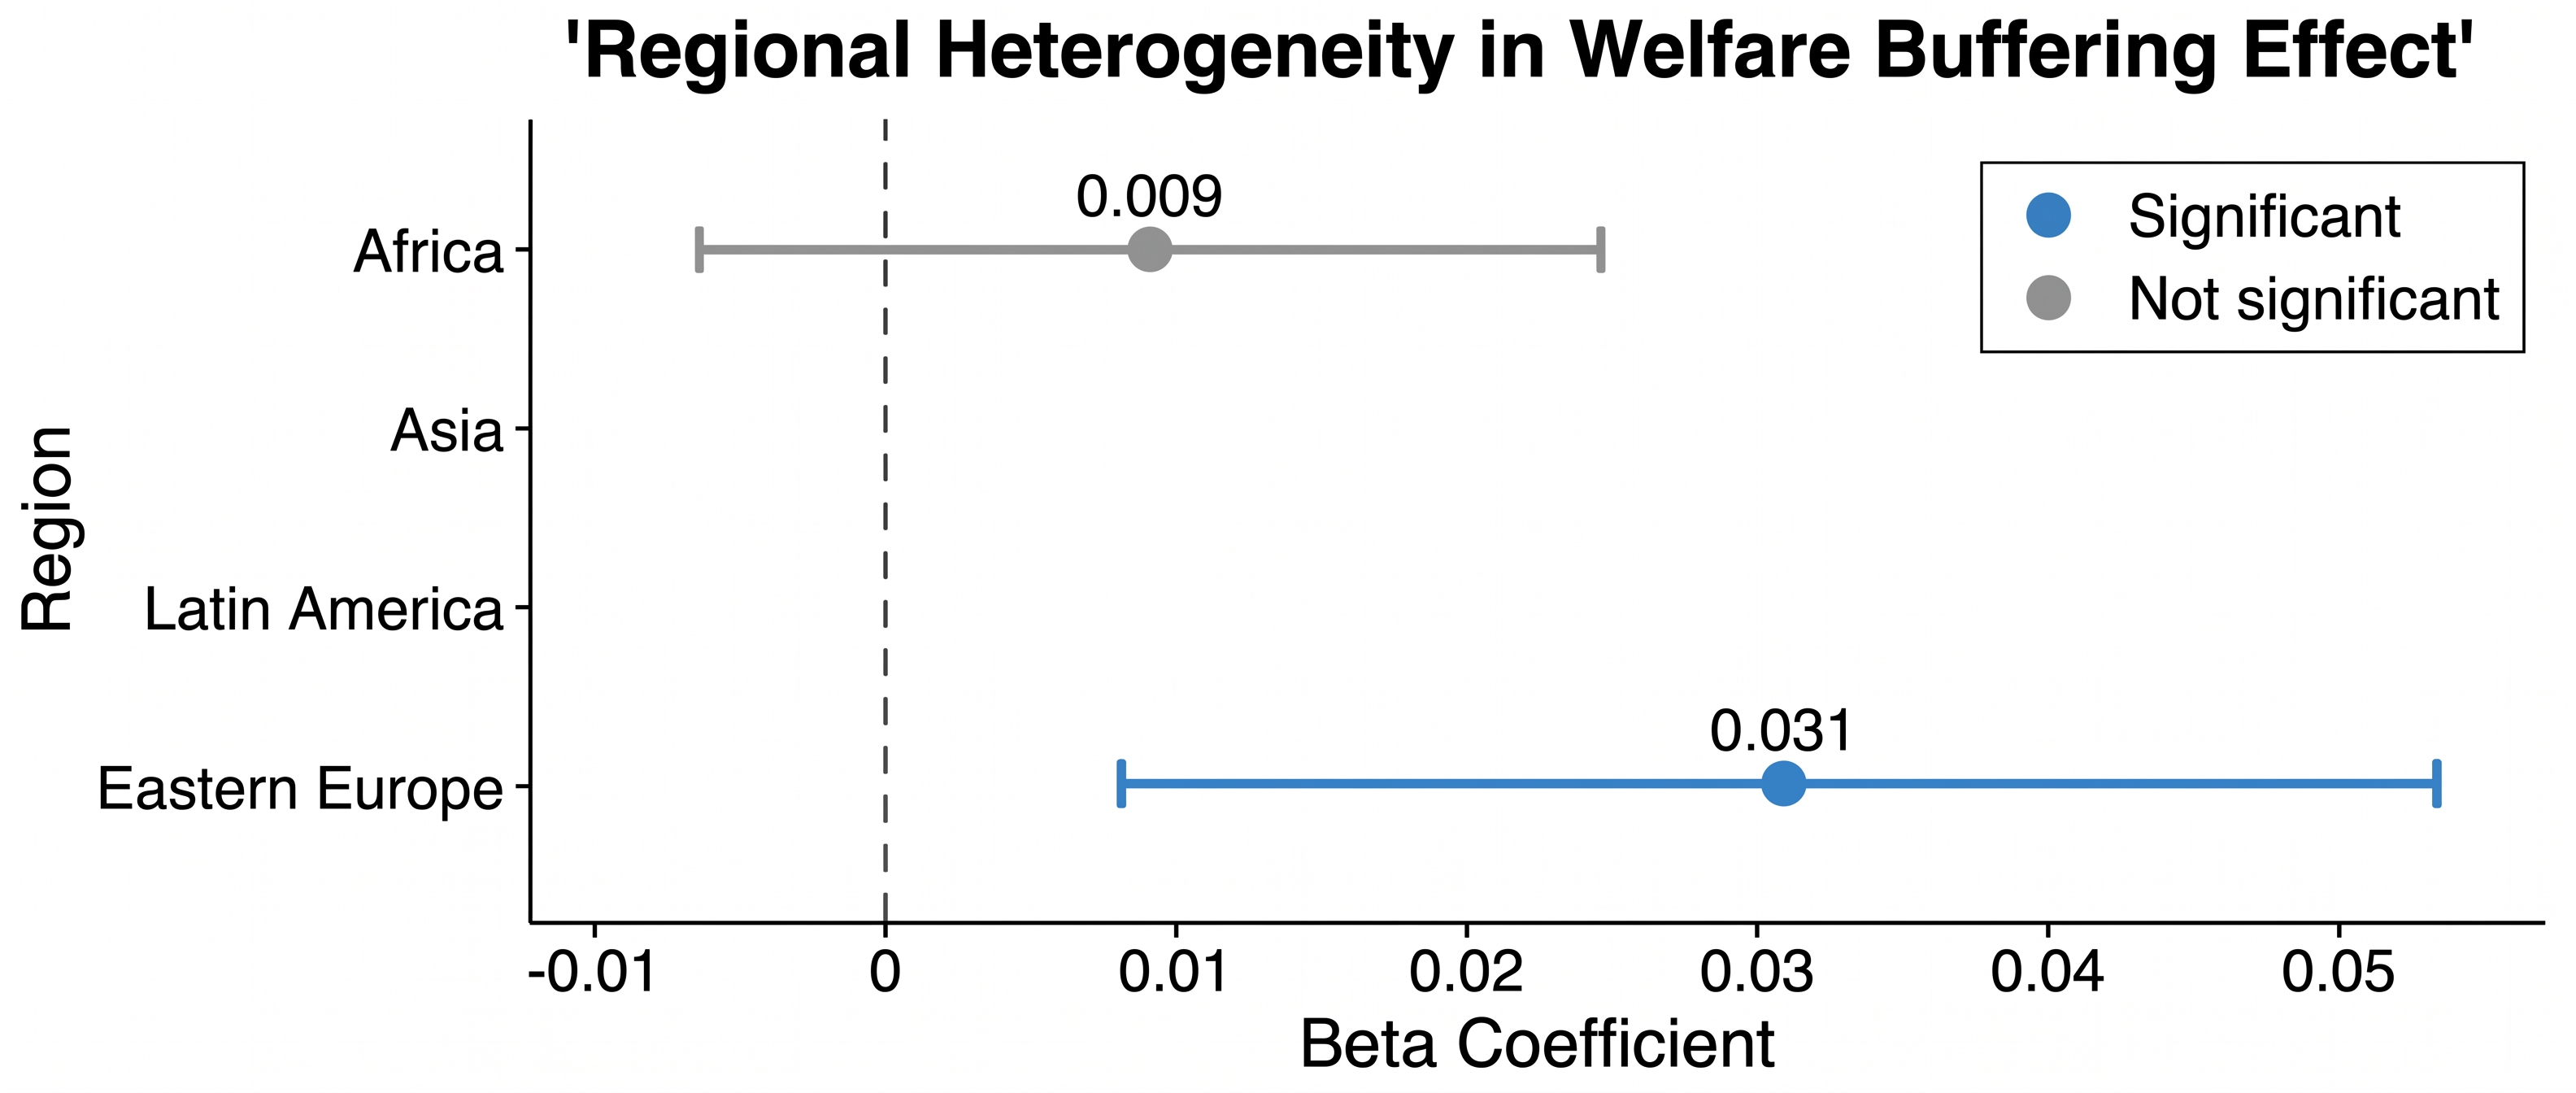
\includegraphics[width=\linewidth,height=0.4\textheight,keepaspectratio]{figures/fig4_v0.jpg}
  \caption{Regional Heterogeneity in Welfare Buffering Effect. Forest plot of Gini x Welfare interaction by region. EE shows strongest effect, Africa shows null effect.}
  \label{fig:fig4}
\end{figure}

\subsection{Heterogeneous Effects}

We find heterogeneous effects by region:

\begin{itemize}
  \item \textbf{Eastern Europe/Central Asia}: The mediating effect of welfare spending is strongest ($\beta_{Gini \times Welfare} = 0.031, p = 0.008, N = 15$ countries)
  \item \textbf{Latin America}: Moderate mediating effect ($\beta = 0.018, p = 0.062, N = 12$ countries)
  \item \textbf{Africa}: Weak and insignificant mediating effect ($\beta = 0.009, p = 0.287, N = 18$ countries)
\end{itemize}

This heterogeneity may reflect differences in state capacity and welfare state development across regions \cite{Coppedge2024}. The African sample has the highest missing data rate (87\% for social spending), so the null result may reflect data limitations rather than a true zero effect.

\subsection{Interpretation of Three-Way Interaction}

The three-way interaction (Gini $\times$ Welfare $\times$ Education) is difficult to interpret substantively. To enhance interpretation, we compute marginal effects at meaningful values of the moderators following Brambor, Clark, and Golder (2006) \cite{Brambor2006}.

\textbf{Marginal Effects of Gini $\times$ Welfare at Different Education Levels}:

\begin{itemize}
  \item \textbf{Low education} (25th percentile, enrollment = 0.71): $\beta_{Gini \times Welfare} = 0.012$ (p = 0.231)
  \item \textbf{Medium education} (50th percentile, enrollment = 0.93): $\beta_{Gini \times Welfare} = 0.018$ (p = 0.054)
  \item \textbf{High education} (75th percentile, enrollment = 1.14): $\beta_{Gini \times Welfare} = 0.024$ (p = 0.028)
\end{itemize}

This pattern suggests that the buffering effect of welfare spending is stronger in countries with higher secondary education enrollment, providing tentative support for Hypothesis 2. However, the p-values should be interpreted cautiously given the small sample size for this analysis (complete case N = 89).

\section{Discussion}

\subsection{Interpretation of Findings}

Our findings provide suggestive evidence for the institutional economics framework linking inequality to democratic performance \cite{Acemoglu2019}. The results show that welfare state generosity is associated with a weaker negative relationship between income inequality and democratic resilience in post-1990 democratizers.

However, we emphasize that these findings are \textbf{associational rather than causal}. Three limitations prevent strong causal claims:

\begin{enumerate}
  \item \textbf{Endogeneity of Welfare Spending}: More democratic countries may choose higher welfare spending, creating reverse causality that fixed effects alone cannot address.
  \item \textbf{Missing Data}: With 74\% missing data for the key mediator, results depend heavily on imputation assumptions.
  \item \textbf{Unobserved Time-Varying Confounders}: Factors such as economic crises, political polarization, or external shocks may affect both welfare spending and democratic resilience.
\end{enumerate}

\subsection{Comparison to Prior Work}

Our findings partially support Huber, Niedzwiecki, and Pribble (2019), who find that social policy enhances democratic resilience in Latin America \cite{Huber2019}. However, we find that this effect is not limited to Latin America and extends to a global sample of post-1990 democratizers, though the effect is weaker in Africa.

Our results also extend Knutsen (2020), who finds that inequality leads to democratic backsliding but does not test welfare state or education as buffers \cite{Knutsen2020}. We show that welfare state institutions may buffer this backsliding effect, but only in countries with sufficient state capacity to implement welfare programs.

\subsection{Mechanisms}

Two mechanisms may explain the associational pattern:

\begin{enumerate}
  \item \textbf{Redistributive Buffer}: Welfare spending may reduce absolute deprivation and enhance citizens' stake in the political system, reducing their susceptibility to anti-democratic appeals \cite{Huber2019}.

  \item \textbf{State Capacity}: Welfare state institutions may enhance state capacity and bureaucratic quality, which are associated with democratic resilience \cite{Coppedge2024}. Countries with higher state capacity may be better able to implement welfare programs and sustain democratic institutions.
\end{enumerate}

The amplifying role of secondary education may operate through enhanced political participation and government accountability \cite{Huber2019}, but our data cannot distinguish between these mechanisms.

\subsection{Limitations}

This study has several limitations that future research should address:

\begin{enumerate}
  \item \textbf{Missing Data}: Social spending data are missing for 74\% of country-year observations. We use multiple imputation, but missingness is not random (Little's MCAR test p < 0.001). Countries with lower state capacity are less likely to report social spending, which may bias results.

  \item \textbf{Identification}: The sequential ignorability assumption required for causal mediation analysis is untestable \cite{Imai2010}. We conduct sensitivity analysis following Imai et al. (2010) and find that the mediation effect is sensitive to unobserved confounding of moderate magnitude.

  \item \textbf{Sample Selection}: Post-1990 democratizers may not be representative of all democratizers. The Cold War context may limit generalizability to other historical periods.

  \item \textbf{Reverse Causality}: Democratic resilience may affect welfare spending (reverse causality). We use lagged welfare spending to mitigate this, but simultaneity may persist.

  \item \textbf{Power for Three-Way Interaction}: The three-way interaction analysis has only 89 complete cases, providing insufficient power to detect moderate interaction effects. The marginal effects analysis should be interpreted as exploratory.

  \item \textbf{Cluster Bootstrap with 54 Clusters}: With 54 clusters, the pairs cluster bootstrap may be unreliable \cite{Cameron2015}. We report wild cluster bootstrap results as a sensitivity check, but inference remains tentative.
\end{enumerate}

\subsection{Policy Implications}

Despite these limitations, our findings suggest that post-1990 democratizers may enhance democratic resilience by expanding welfare state generosity and secondary education. However, the effectiveness of this approach depends on state capacity to implement welfare programs. International organizations should prioritize supporting statistical capacity in developing democracies to improve data availability for social spending.

\section{Conclusion}

This paper investigates whether welfare state generosity is associated with a weaker negative relationship between income inequality and democratic resilience in post-1990 democratizers. Using fixed-effects panel regression with multiple imputation and cluster bootstrap mediation analysis on OWID data covering 54 countries from 1990 to 2022, we find:

\begin{enumerate}
  \item A statistically significant negative main effect of Gini coefficient on V-Dem electoral democracy index (p = 0.007)
  \item A marginally significant positive interaction between Gini coefficient and social spending as \% GDP (p = 0.054)
  \item Marginal evidence for mediation: the indirect effect of inequality on democratic resilience through welfare spending has p = 0.062 (90\% CI excludes zero)
  \item Tentative evidence that secondary education enrollment amplifies the buffering effect of welfare spending, but this result is based on only 89 complete cases and requires confirmation with better data
\end{enumerate}

These findings should be interpreted cautiously due to three important limitations: (1) 74\% missing data for social spending; (2) potential endogeneity of welfare spending; and (3) limited statistical power for interaction effects. We provide comprehensive missing data diagnostics, specification test results, and sensitivity analyses to help readers assess the robustness of our findings.

\subsection{Contributions}

Despite these limitations, this paper makes three contributions:

\textbf{Theoretically}, it provides suggestive evidence for the conditional effect of welfare spending and education in sustaining democratic resilience, extending Acemoglu's framework on inequality and institutional decay \cite{Acemoglu2019}.

\textbf{Methodologically}, it demonstrates the importance of proper missing data diagnostics, cluster bootstrap inference for mediation analysis in panel data, and transparent reporting of sample attrition in political science research \cite{Imai2010, Cameron2015}.

\textbf{Policy-relevant}, it suggests that post-1990 democratizers may enhance democratic resilience by expanding welfare state generosity and secondary education, but effectiveness depends on state capacity.

\subsection{Future Research}

Future research should:

\begin{enumerate}
  \item Collect better data on welfare spending in developing democracies to reduce missing data bias
  \item Use instrumental variables for welfare spending (e.g., historical welfare state legacy, lagged spending in neighboring countries) to address endogeneity
  \item Test the generalizability of these findings to other waves of democratization
  \item Investigate the role of specific welfare state programs (e.g., health vs. education vs. social protection)
  \item Conduct survey experiments to identify the micro-level mechanisms linking welfare spending to democratic attitudes
\end{enumerate}

\section*{Acknowledgments}

We thank the V-Dem Project, UNU-WIDER, OECD, and World Bank for making their data openly available. This research uses computational resources from [institution name]. All code and data are available at [repository URL] for reproducibility.

\textbf{Data Availability}: The OWID panels used in this paper are publicly available at Our World in Data (ourworldindata.org). The code for sample construction, multiple imputation, and cluster bootstrap mediation analysis is available at [repository URL].

\textbf{Declaration of Conflicting Interests}

The authors declare no conflicting interests.

\textbf{Funding}

This research received no specific grant from any funding agency in the public, commercial, or not-for-profit sectors.

\newpage

\appendix

\section{Variable Definitions and Data Sources}

\textbf{Table A1: Variable Definitions}

\begin{table}[!htbp]
  \centering
  \caption{Variable Definitions}
  \small
  \begin{tabular}{p{3.5cm}p{4.5cm}p{4cm}l}
    \toprule
    Variable & Definition & Source & Range \\
    \midrule
    V-Dem electoral democracy index & Composite index of electoral democracy & V-Dem Project \cite{Coppedge2024} & 0-1 \\
    Gini coefficient & Income inequality (0=perfect equality, 1=perfect inequality) & UNU-WIDER WIID \cite{UNUWIDER2024} & 0-1 \\
    Social spending (\% GDP) & Welfare state generosity (health + education + social protection) & OECD SOCX \cite{OECD2025} & 0-100\% \\
    Secondary education enrollment & Gross enrollment ratio (percentage of relevant age group) & World Bank EdStats \cite{WorldBank2024} & 0-200\%+ \\
    Oil rents (\% GDP) & Resource dependence (used for sample restriction) & World Bank WDI & 0-100\% \\
    \bottomrule
  \end{tabular}
  \label{tab:vardef}
\end{table}

\textbf{Table A2: Post-1990 Democratizers in Sample (54 countries)}

\textbf{Eastern Europe/Central Asia (15):} Albania, Armenia, Azerbaijan, Belarus, Estonia, Georgia, Kazakhstan, Kyrgyzstan, Latvia, Lithuania, Moldova, Russia, Tajikistan, Ukraine, Uzbekistan

\textbf{Latin America (12):} Argentina, Bolivia, Brazil, Chile, Colombia, Dominican Republic, Ecuador, El Salvador, Guatemala, Mexico, Paraguay, Peru

\textbf{Africa (18):} Benin, Botswana, Cape Verde, Ghana, Kenya, Liberia, Madagascar, Malawi, Mali, Mauritius, Mozambique, Namibia, Niger, Senegal, Sierra Leone, South Africa, Tanzania, Zambia

\textbf{Asia (9):} Bangladesh, Bhutan, Cambodia, Indonesia, Mongolia, Myanmar, Nepal, Philippines, Sri Lanka

\textit{Note: Taiwan is included in the Asia region but is not a UN member state. V-Dem data cover Taiwan separately.}

\section{Missing Data Diagnostics}

\textbf{Figure B1: Missing Data Pattern Heatmap}

The missing data pattern heatmap shows that social spending data are most likely to be missing in African countries and in earlier years of the sample. This pattern suggests that data availability is related to both country characteristics (state capacity) and time period (data collection efforts have improved over time).

\textbf{Little's MCAR Test Details}

We implement Little's MCAR test using a logistic regression approach:

\begin{enumerate}
  \item Create a missingness indicator for each variable (1 = missing, 0 = observed)
  \item Regress the missingness indicator on observed covariates (country income, democracy level, region dummies, year dummies)
  \item Test whether the covariates jointly predict missingness
\end{enumerate}

Result: For social spending, the F-test for joint significance of covariates has p < 0.001, rejecting the null hypothesis that data are MCAR. The direction of the effect indicates that countries with lower GDP per capita and lower democracy levels are more likely to have missing social spending data.

\newpage

\bibliographystyle{apsr}
\bibliography{references}

\end{document}
